\section{Introduction}

White Rabbit (WR, \cite{biblio:whiteRabbit}) is a project which aims at creating an
Ethernet-based network with low-latency, deterministic packet delivery
and network-wide, transparent, high-accuracy timing distribution. The
White Rabbit Network (WRN) is based on existing standards, namely
Ethernet (IEEE 802.3 \cite{biblio:IEEE8023}), Synchronous Ethernet
(SyncE \cite{biblio:SynchE}) and PTP \cite{biblio:IEEE1588}. 
It is fully compatible with these standards.

A WRN consists of White Rabbit Nodes (nodes) and White Rabbit Switches
(switches) interconnected by fiber or copper links. 
\modified{The focus of this article is on 1000Base-LX \cite{biblio:IEEE1588} 
single-mode fiber connections only. WR }%It also
supports integration of nodes and/or switches that are not White Rabbit. 
A simple WRN is presented in \figurename~\ref{fig:WRnetwork}.

A node is considered the source and destination of information sent
over the WRN. The information distributed over a WRN includes:
\begin{itemize}
   \item  Timing - frequency and International Atomic Time (TAI).
   \item  Data  - Ethernet traffic between nodes.
\end{itemize} 

In order to understand the goals of the WR project -- namely
determinism, high reliability and accurate synchronization -- these
terms are explained below.

\textbf{Determinism} is guaranteed by having a worst-case upper bound
in frame delivery latency.  

\textbf{Accuracy} is a measure of the deviation between the clock of
the \textit{grandmaster} node\modified{/switch} of a WRN and that of any other node.
Assuming only fiber interconnections, a WRN is meant to achieve
sub-nanosecond accuracy. 

\textbf{Reliability} of a WRN refers to robust delivery of data and
timing to all the nodes.
% data being delivered in a deterministic manner. 
%A WRN is considered reliable only if all the nodes, receive
%data and timing. 
The timing must allow all the nodes to be
synchronized with the required accuracy and the data must always be
delivered on time.
\begin{figure}[!t]
\centering
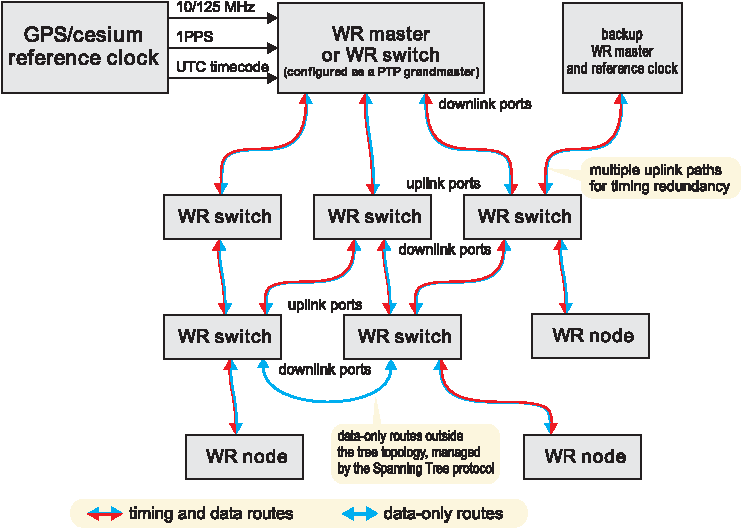
\includegraphics[height=2.10in]{network/hierarchy.eps}
\caption{A White Rabbit Network \cite{biblio:TomekMSc}.}
\label{fig:WRnetwork}
\end{figure}

All these features are required to create a timing and control system which may
replace the General Machine Timing (GMT) \cite{biblio:GMT} at CERN and
fulfill a similar role at the Facility for Antiproton and Ion
Research (FAIR) in GSI \cite{biblio:FAIRtimingSystem}. Such system requires 
synchronization of up to 2000 nodes with sub-nanosecond accuracy, 
an upper bound in frame delivery and a very low data loss rate.
However, many other applications of White Rabbit are possible. This includes industry,
telecommunications and other large distributed systems (e.g. distributed
oscilloscopes \cite{biblio:distOscilloscope}).

This article focuses solely on the PTP-based timing distribution in a WRN. PTP is a packet-based
protocol designed to synchronize devices in distributed systems. The accuracy of the PTP
synchronization is implementation-dependent. The standard is foreseen for 
% this is how I understand the fact that corretionField can carry fractional
% nanoseconds and the syncEventEgressTimestamp includes this figures (see e.g.: 
% clause 9.5.9.3, page 103 of PTP
sub-nanosecond accuracies. However, such performance is not achieved in typical PTP
implementations for two reasons:
\begin{itemize}
  \item Limited precision and resolution of PTP timestamps.
  \item Unknown physical link asymmetry. 
\end{itemize}
Additionally, the quality of PTP-syntonization depends on the exchange rate 
of PTP messages. The higher the quality of the clock we want to recover, 
the higher the bandwidth needed for PTP-related traffic.

The precision of timestamps is greatly increased in the existing PTP implementations
by hardware-based timestamping. However, such implementations
are limited by the resolution which is specified by the hardware-driving frequency
(e.g. 8ns for 125MHz).

The asymmetry is not detectable by PTP; if known, PTP corrects for it to increase
synchronization accuracy. Some of the sources of the physical layer asymmetry can be
eliminated by proper network configuration, e.g. excluding routers or non-PTP bridges from the
network. Others, in particular the inaccuracy caused by physical medium asymmetry (i.e.
difference in propagation velocity in two-way communication over fiber) or PCB layout (i.e.
connection length between PHY and timestamping hardware) need to be obtained through proper a
priori-measurement. 

White Rabbit addresses these limitations to achieve sub-nanosecond accuracy
of synchronization. It uses SyncE to distribute the common notion of frequency in the entire
network over the physical medium. It casts the problem of timestamping into a phase detection
measurement. The results of these precise measurements are used both during normal PTP operation
and for quantifying physical medium asymmetry during the calibration phase.
% Consequently, high precision
% timestamps are obtained. Moreover, the parameters necessary to calculate the physical medium
% asymmetry can be determined. 
%This knowledge is used in the PTP computations of the clock offset and link delay. 
The improved performance of the synchronization is accomplished without increasing PTP-related
traffic (it can be actually decreased) since PTP is only governing the synchronization, while the
syntonization is done by SyncE.

A great effort has been made to align WR-specific solutions with the PTP standard and stay fully
compatible with PTP gear. Consequently, WR can be seen as an extension to PTP. This extension,
called WRPTP, defines its own PTP profile and describes all the WR-specific mechanisms which need
to be implemented by a node/switch to enable sub-nanosecond synchronization with another 
nodes/switches. 
\modified{The compatibility with PTP makes WR more likely to be used in existing PTP-based 
systems by gradual and/or partial upgrade to WRPTP. It also enables the creation of hybrid, 
thus cost-effective, systems.}
WRPTP is presented in section~\ref{sec:wrptp} \textit{White Rabbit PTP}.
Section~\ref{sec:hwSupport} presents an example implementation of 
hardware which supports WRPTP. Finally, the measurements of WRPTP performance and conclusions are
presented in the last two sections of this article.

In PTP nomenclature, the main component of a WRN, the switch, is a boundary clock (BC) -- a clock 
that has multiple PTP ports. Similarly, the node is an ordinary clock (OC) --
a clock that has a single PTP port. Consequently, the WRN
can be seen as a set of independently synchronized Master-to-Slave
(M-to-S) links with ports of OC or BC on both sides
(\figurename~\ref{fig:WRnetwork}, red-blue arrows). The ability to
synchronize a single link scales into the ability to synchronize the
entire network. Therefore, in this article, only a single M-to-S link is
considered, where appropriate.


